\chapter{Background}
To understand the details of how Explorant works, we will provide context on certain aspects of the stack that are particularly important for understanding its functionality. Namely, we describe how debuggers help with code understanding, what a state diagram is, and how RR \cite{rr-site} works. 

\section{Debuggers and Breakpoints}
\label{sec:debuggers}
Debuggers are an essential tool for software developers, as they allow us to pause the execution of a program and inspect its state at any given moment. This is useful for detecting and fixing bugs, as well as for understanding how the program works. GDB \cite{gdb} is one of the most widely known debuggers for statically compiled languages (i.e. not interpreted languages like Javascript). GDB allows a developer to step through a program line by line to see the exact execution path. A developer normally uses a tool like GDB when they know a little bit about how a program works but they are looking to solidify their knowledge and dive deeper. 

One of the most important things debuggers can do is set \textit{software-breakpoints}. These work by replacing the first byte of an instruction with 0xcc, also known as \texttt{INT3} \cite{int3}. When this instruction is executed, the CPU throws an \texttt{EXCEPTION\_BREAKPOINT} which calls the debugger's exception handler. This allows the debugger to fix the first byte of the instruction and modify the instruction pointer register to act as if the instruction had never been run. At this point, the debugger has full access to the program's memory and the developer can do things like examine memory addresses and data structures. Explorant utilizes this technique to allow the developer to open GDB at any specific instance in time. 

\section{State Machines and Diagrams}
\label{sec:fsm}

\begin{figure}[!ht]
\centering
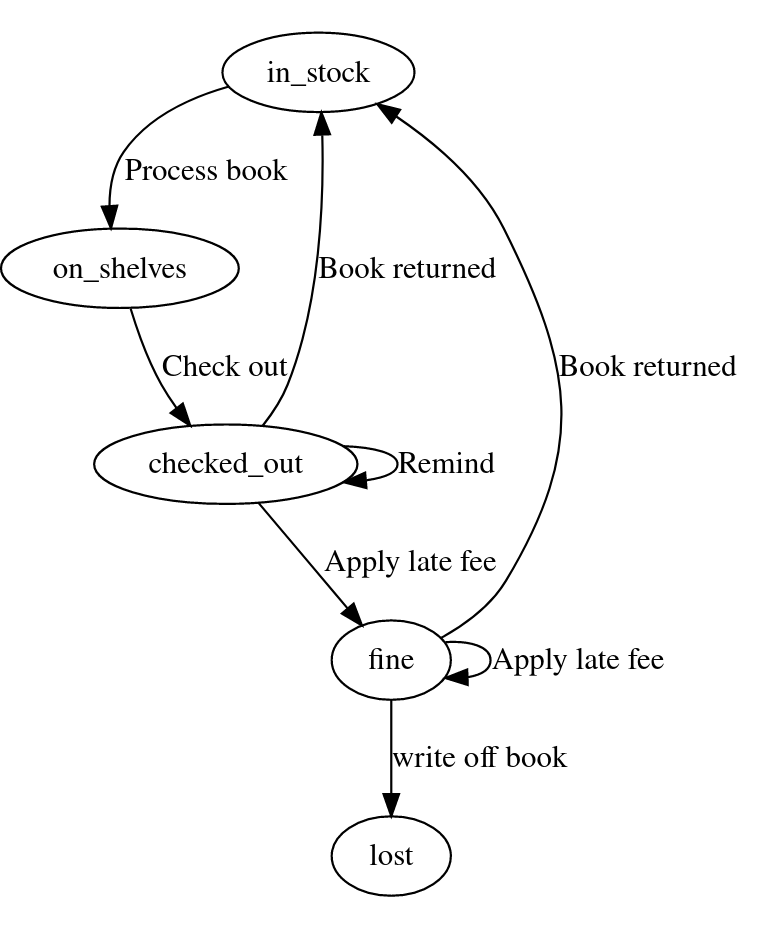
\includegraphics[scale=0.5]{state-book}
    \caption{Simple state diagram of a library bookkeeping system}
    \label{fig:state-book}
\end{figure}

State diagrams are directed graphs that help programmers condense lots of complicated domain knowledge into a small number of states. These diagrams show how the states of a program relate to each other \cite{state}. State diagrams are particularly useful for onboarding new developers, as they provide a high-level overview of the program's flow without requiring a deep understanding of the code \cite{onboarding-ramp, state}.


Each node in a state diagram represents a unique state of the program and each edge represents an action that can occur to transition states. For example, in figure \ref{fig:state-book}, a book in the \texttt{checked\_out} state can be returned, the person can be reminded, or the person can get a late fee. 


Finite state machines (FSMs) are visually similar to state diagrams but they apply the node transitions with more rigor \cite[p~55]{fsm}. FSMs specify all of the conditions that lead to a transition and have no concept of global state. They are a very limited concept of computation. Explorant does not directly generate FSMs however it uses graph mining techniques to estimate what an FSM of a given program could look like (See section \ref{sec:synoptic}).


% \begin{figure}
% \centering
% \begin{tikzpicture}[node distance=4.5 cm]
% \node[rectangle, draw] (A) {Idle};
% \node[rectangle, draw] (B) [right of=A] {Listening for user input};
% \node[rectangle, draw] (C) [below of=B] {Processing user input};
% \node[rectangle, draw] (D) [below of=C] {Generating response};
% \node[rectangle, draw] (E) [left of=C] {Sending response};
% \draw [->, =>stealth] (A) -- (B);
% \draw [->, =>stealth] (B) -- (C);
% \draw [->, =>stealth] (C) -- (D);
% \draw [->, =>stealth] (D) -- (E);
% \draw [->, =>stealth] (E) -- (A);
% \end{tikzpicture}
% \caption{Simple state diagram for a bot}
%     \label{fsm:unlabeled}
% \end{figure}


\textit{Explorant does not use traditional state diagrams as we do not have the ability to intelligently label edges}. All of the state diagrams that Explorant can generate are unlabeled (this may change in the future). However, using techniques described in the graph simplification (\ref{sec:simplification}) section, we are still able to ensure that the graph is both understandable and usable. 

\section{ELF / DWARF}
The ELF (Executable and Linkable Format)\cite{elf-book} is a file format used by many Unix-like operating systems to specify the layout of object files and executables. These files contain a wealth of information about the compiled code, including symbols, debugging information, and other metadata.

One component of ELF files is DWARF (Debugging With Attributed Record Formats)\cite{dwarf-site}, which is a data format that specifies the layout of debugging information. DWARF data is embedded in ELF files and can be accessed by debuggers, such as GDB, to provide valuable information about the execution of a program.

DWARF data is organized into structures called DIEs (Debugging Information Entries), which are composed of key value pairs for the structures in the original source file. Some common DIE tags include \texttt{DW\_TAG\_variable} for variables, \texttt{DW\_TAG\_subprogram} for functions, and \texttt{DW\_TAG\_compile\_unit} for compilation units. You can see table \ref{fig:subprogram_die} to see all of the information that goes into one of these DIE entries for a function.  

\begin{table}
\centering
    \begin{tabular}{l|l}
\textbf{Attribute} & \textbf{Description} \\ \hline
        DW\_AT\_external & Whether the function was defined in this program (ex: printf is external)\\ 
DW\_AT\_name & The name of the subprogram \\ 
DW\_AT\_decl\_file & The path to the souce file where this function was defined \\ 
DW\_AT\_decl\_line & Line in the source file where this function was defined\\ 
DW\_AT\_decl\_column & Column in the source file where this function was defined\\ 
DW\_AT\_type & Return type of the function \\ 
DW\_AT\_low\_pc & The starting address of the subprogram \\ 
DW\_AT\_high\_pc & The ending address of the subprogram \\ 
DW\_AT\_prototyped & Specifies whether the subprogram has a prototype \\ 
\end{tabular}
\caption{A table of attributes for a DW\_TAG\_subprogram DIE.}
    \label{fig:subprogram_die}
\end{table}

By parsing out these DIE tags, Explorant can access valuable information about the symbols in a program, allowing us to provide useful features such as the ability to correlate lines of code with addresses and figure out which function a particular line is a part of. 

\section{RR Record and Replay Framework}
Explorant uses RR \cite{rr-site} extensively and would not be possible without it. The RR record and replay framework is a powerful extension to GDB that enables the user to \textit{continue backwards} as well as forwards while debugging \cite{rr-site}. This allows user to easily and quickly reproduce the conditions that led to a bug. This is particularly useful when debugging rare or timing-sensitive bugs like race conditions where GDB might prevent the bug from ever occurring in the first place.

One key aspect of RR is its focus on capturing nondeterministic input rather than the whole trace \cite{rr-site}. In this case, nondeterministic inputs are the events that could cause a program's output to vary from run to run. This includes things like syscall inputs and outputs, process-switching timings, or even some non-deterministic instructions. By capturing and replaying these inputs, RR avoids having to walk through and instrument the vast majority of executed instructions. RR uses a wide variety of tools including the \texttt{ptrace} API \cite{ptrace-site} to attach middleware, overwriting the vDSO (virtual dynamic shared object), limiting a program to a single core, and other more specific techniques in order to accomplish record and replay. 

To intercept many simple system calls, RR can simply overwrite the vDSO which is a user-space code-segment that the kernel exports for code ``that does not necessarily have to run in kernel space'' \cite{vdso}. However some code can directly execute syscalls in assembly. As such, ``when the tracee makes a system call, RR is notified via a ptrace trap and it tries to rewrite the system-call instruction to call into [their] interception library'' \cite[p.~8]{rr}. A diagram of this modification can be seen in figure \ref{fig:subprogram_die}. A similar process happens during replay and all of the nondeterministic calls are replaced with lookups to get the deterministic input from the recording.

\begin{figure}
\centering
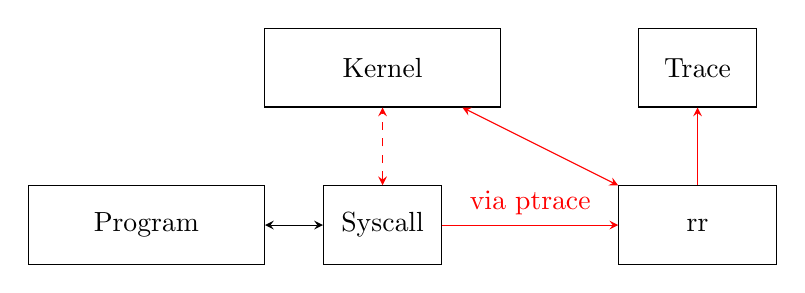
\begin{tikzpicture}

%RR
\node[rectangle, draw, minimum width=2cm, minimum height=1cm] (rr) at (7,-2) {rr};

%Kernel
\node[rectangle, draw, minimum width=3cm, minimum height=1cm] (kernel) at (3,0) {Kernel};

%Program
\node[rectangle, draw, minimum width=3cm, minimum height=1cm] (program) at (0,-2) {Program};

%VDSO
\node[rectangle, draw, minimum width=1.5cm, minimum height=1cm] (syscall) at (3,-2) {Syscall};

%Trace
\node[rectangle, draw, minimum width=1.5cm, minimum height=1cm] (trace) at (7,0) {Trace};

%System Call
\draw[<->, >=stealth] (program) -- (syscall);
\draw[<->, >=stealth, red, dashed] (syscall) -- (kernel);
\draw[<->, >=stealth, red] (rr) -- (kernel);
\draw[->, >=stealth, red] (syscall) -- (rr) node[midway,above ] {via ptrace};
\draw[->, >=stealth, red] (rr) -- (trace);

\end{tikzpicture}
\caption{Diagram showing how RR intercepts calls into the kernel and records them}
\end{figure}


    In order to efficiently \textit{continue-backwards}, RR utilizes a checkpointing system. The checkpointing system works by \texttt{fork}ing the process to cheaply copy the address space \cite[p.~15]{rr}. This is efficient because ``fork is (mostly) 'copy-on-write' and is very well optimized on Linux, so creating a checkpoint typically takes less than ten milliseconds'' \cite[p.~15]{rr}. This allows RR to quickly and easily restore the program to the state it was in at the time of the checkpoint. Then it can continue-forwards until it reaches the desired location.

The default interface to RR is a GDB server using the GDB remote serial protocol \cite{gdb-proto}. However, this is not a performant solution for a programmatic interface that might be doing queries across the entire execution of a program. As such, we developed \textit{librr}, a Rust library to interact with the C++ internals and provide nice abstractions such as reading registers, writing bytes in memory, setting breakpoints, etc. 



